\documentclass[a4paper,11pt]{article}

\usepackage[portuguese]{babel}
\usepackage[utf8]{inputenc}
\usepackage{amsmath}
\usepackage{graphicx}
\usepackage{hyperref}
\usepackage{float}
\usepackage{subfig}
\usepackage{fixltx2e}
\usepackage[bottom]{footmisc}
\usepackage{listings}
\usepackage{color} 
\usepackage[usenames,dvipsnames]{xcolor}
\usepackage[colorinlistoftodos]{todonotes}
\usepackage[font=footnotesize]{caption}

\usepackage[hypcap]{caption}
\usepackage[top=2.5cm, bottom=2.5cm, left=2.5cm, right=2.5cm]{geometry}
\usepackage{enumerate}

\numberwithin{equation}{section}
\addto\captionsportuguese{\renewcommand{\contentsname}{Índice}}

\linespread{1.3}
\usepackage{indentfirst}

\begin{document}
\begin{titlepage}
\begin{center}
	
\hfill \break
\hfill \break


\includegraphics[width=0.3\textwidth]{img/logo}~\\[1cm] 

\textsc{\LARGE Instituto Superior Técnico}\\[0.25cm]
\textsc{\Large Mestrado Integrado em Engenharia Electrotécnica e de Computadores}\\[1.8cm]
\textsc{\huge Electrónica de Potência}\\[0.25cm]

\vspace{6mm}

{\huge \bfseries Circuito de Disparo de um Tiristor \linebreak \& \linebreak Circuito com Carga Ressonante \linebreak Comutação pela Carga  \\[1cm]}

\begin{tabular}{ l l }
	João Bernardo Sequeira de Sá & \hspace{2mm} n.º 68254 \\
	Maria Margarida Dias dos Reis & \hspace{2mm} n.º 73099 \\
	Rafael Augusto Maleno Charrama Gonçalves & \hspace{2mm} n.º 73786 \\
	Nuno Miguel Rodrigues Machado & \hspace{2mm} n.º 74236
\end{tabular}

\vspace{7mm}

Grupo n.º TAL de segunda-feira das 17h00 - 2000

\vfill

{\large Lisboa,  de  de 2015} 
	
\end{center}
\end{titlepage}
	
\tableofcontents
\pagebreak

\section{Introdução}

Pretende-se com este trabalho estudar o comportamento do tiristor, com especial interesse na passagem à condução e ao corte deste dispositivo, assim como evidenciar alguns aspetos da sua utilização em circuitos de conversão de potência.

O tiristor, ou retificador controlado de silício, é o dispositivo indicado para comandar tensões e correntes de valor elevado, sendo capaz de suportar potências da ordem dos 10 MW. É composto por três terminais, o elétrodo de disparo, ou \textit{gate} (G), ânodo (A) e cátodo (K). Através da \textit{gate} pode levar-se o dispositivo à condução, caso este esteja polarizado diretamente nos terminais de ânodo e cátodo, através de um impulso. 

Por norma, os terminais de potência, ânodo e cátodo, desempenham funções semelhantes aos terminais do díodo. Em oposição ao transístor, o tiristor é um dispositivo que possui memória; uma vez que seja colocado à condução não regressa ao estado de bloqueio através de atuação na gate, mas sim através de um anulamento da corrente, polarização inversa, comportamento idêntico ao do díodo. Gera-se assim uma necessidade para que, caso o circuito em que o dispositivo é aplicado não possua uma comutação natural, se recorra a técnicas de comutação forçada.

Estas técnicas de comutação forçada são concebidas normalmente com recurso a componentes reativos, como sejam a bobine ou o condensador, para que possa ser estabelecida uma polarização inversa aos terminais do tiristor num certo período de tempo do funcionamento do circuito. Estas técnicas levam no entanto a perdas, pelo que as frequências de operação são da ordem de 500 a 1.5 kHz.

Atualmente existe tendência para usar como alternativa IGBT's ou GTO's.

\pagebreak

\section{Circuito de Disparo}

De forma a estudar o comportamento de circuitos com semicondutores de potência é necessário, em primeira instância, realizar o circuito de “drive” ou ataque ao terminal de controlo ou, no caso de tiristores, o circuito de disparo. Este circuito tem a função de estabelecer o sinal de comando do tiristor, sendo este aplicado entre a \textit{gate} e o cátodo, assim como estabelecer o isolamento galvânico entre o circuito de potência e o circuito de controlo. Pode observar-se este circuito na \autoref{fig:circuit_1}.

\begin{figure}[h]
	\centering
	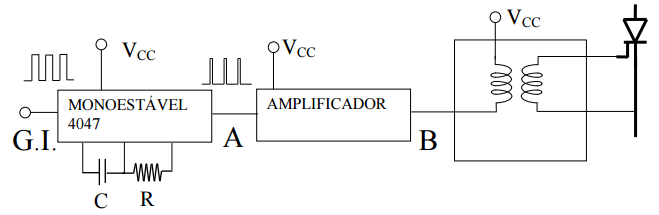
\includegraphics[keepaspectratio=true, scale=0.37]{teoricas/trigger_circuit}
	\caption{Circuito de disparo.}
	\label{fig:circuit_1}
	\vspace{-0.8em}
\end{figure}

O objetivo neste trabalho é assim realizar este circuito com uma frequência de 2 kHz, fazendo para isso uso de um sinal com esta frequência originado por um gerador de impulsos (GI). O circuito de disparo será então composto por uma monoestável que reage ao flanco ascendente do sinal originado pelo GI; tem-se assim à saída da monoestável um impulso cuja duração será função da resistência $R$ e condensador $C$. 

A duração deste impulso deve ser definida consoante as características da \textit{gate} do tiristor que se está a utilizar, sendo neste caso de 10 $\mu$s. Este impulso tem, no entanto, que ser amplificado para que seja injetada corrente suficiente na \textit{gate} do tiristor. Usa-se assim um transístor de ganho elevado transitando da saturação ao corte, estabelecendo uma tensão no primário do transformador, sempre que surja o impulso na saída da monoestável. As formas de onda destes impulsos podem ser observadas na \autoref{fig:circuit_2}.

\begin{figure}[h]
	\centering
	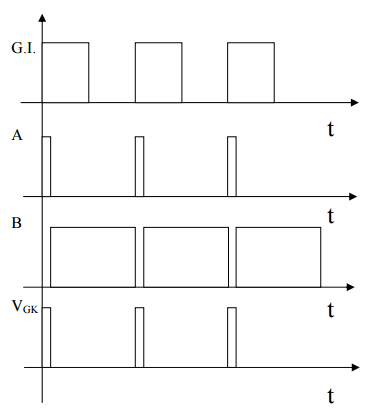
\includegraphics[keepaspectratio=true, scale=0.45]{teoricas/trigger_waveform}
	\caption{Formas de onda das tensões no circuito de disparo.}
	\label{fig:circuit_2}
	\vspace{-0.8em}
\end{figure}

O transformador serve também para que se obtenha o isolamento galvânico entre os circuitos de disparo e de potência.

\pagebreak

\section{Montagem e equipamento}

A montagem presente na placa impressa utilizada no laboratório pode ser observada na \autoref{fig:circuit_3}.

\begin{figure}[h]
	\centering
	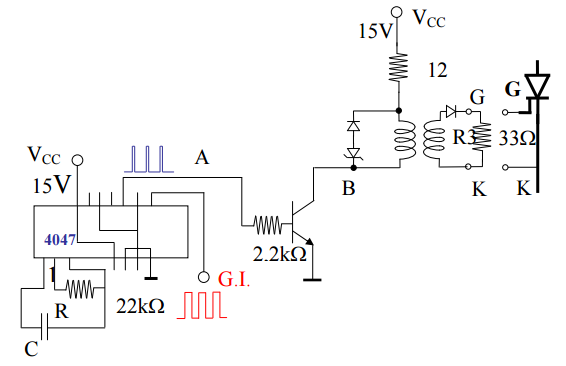
\includegraphics[keepaspectratio=true, scale=0.45]{teoricas/assembly_circuit}
	\caption{Esquema elétrico do circuito de disparo presente na placa impressa.}
	\label{fig:circuit_3}
	\vspace{-0.8em}
\end{figure}

Tal como dito na secção acima, a duração do impulso, $T$, será definida pela resistência $R$ e o condensador $C$ segundo a seguinte fórmula dada pelo fabricante.

\vspace{-3mm}
\begin{equation}
T = 2.88 \ RC.
\end{equation}

Para que se tenha 10 $\mu$s faz-se assim uso de uma resistência com $10$ k$\Omega$ e $0.4$ nF, sem necessidade de uma grande precisão nos valores, pois a exatidão do tempo de disparo neste circuito não é prevalente.

O equipamento a utilizar na condução do trabalho é assim:

\vspace{-2mm}

\begin{itemize}
	\item 1 osciloscópio;
	\vspace{-2mm}	
	\item 1 sonda de corrente;
	\vspace{-2mm}	
	\item 1 gerador de impulsos;
	\vspace{-2mm}	
	\item 2 fontes de alimentação;
	\vspace{-2mm}	
	\item 2 multímetros;
	\vspace{-2mm}	
	\item 1 placa de circuito impresso.
\end{itemize}

\pagebreak

\section{Condução do Trabalho}

\subsection{circuito de disparo}

Em primeira instância apenas se realizam as ligações do circuito de disparo à fonte de alimentação. Após as ligações feitas sintoniza-se o GI para que se obtenha na saída uma onda retangular de amplitude $0$ a $15$ a uma frequência de $1$ kHz com fator de ciclo de 50\%.

Feito isto podem observar-se as formas de onda entre o ponto A e a massa e o ponto B e a massa no osciloscópio tal como na \autoref{fig:photo 1}

\begin{figure}[h]
	\centering
	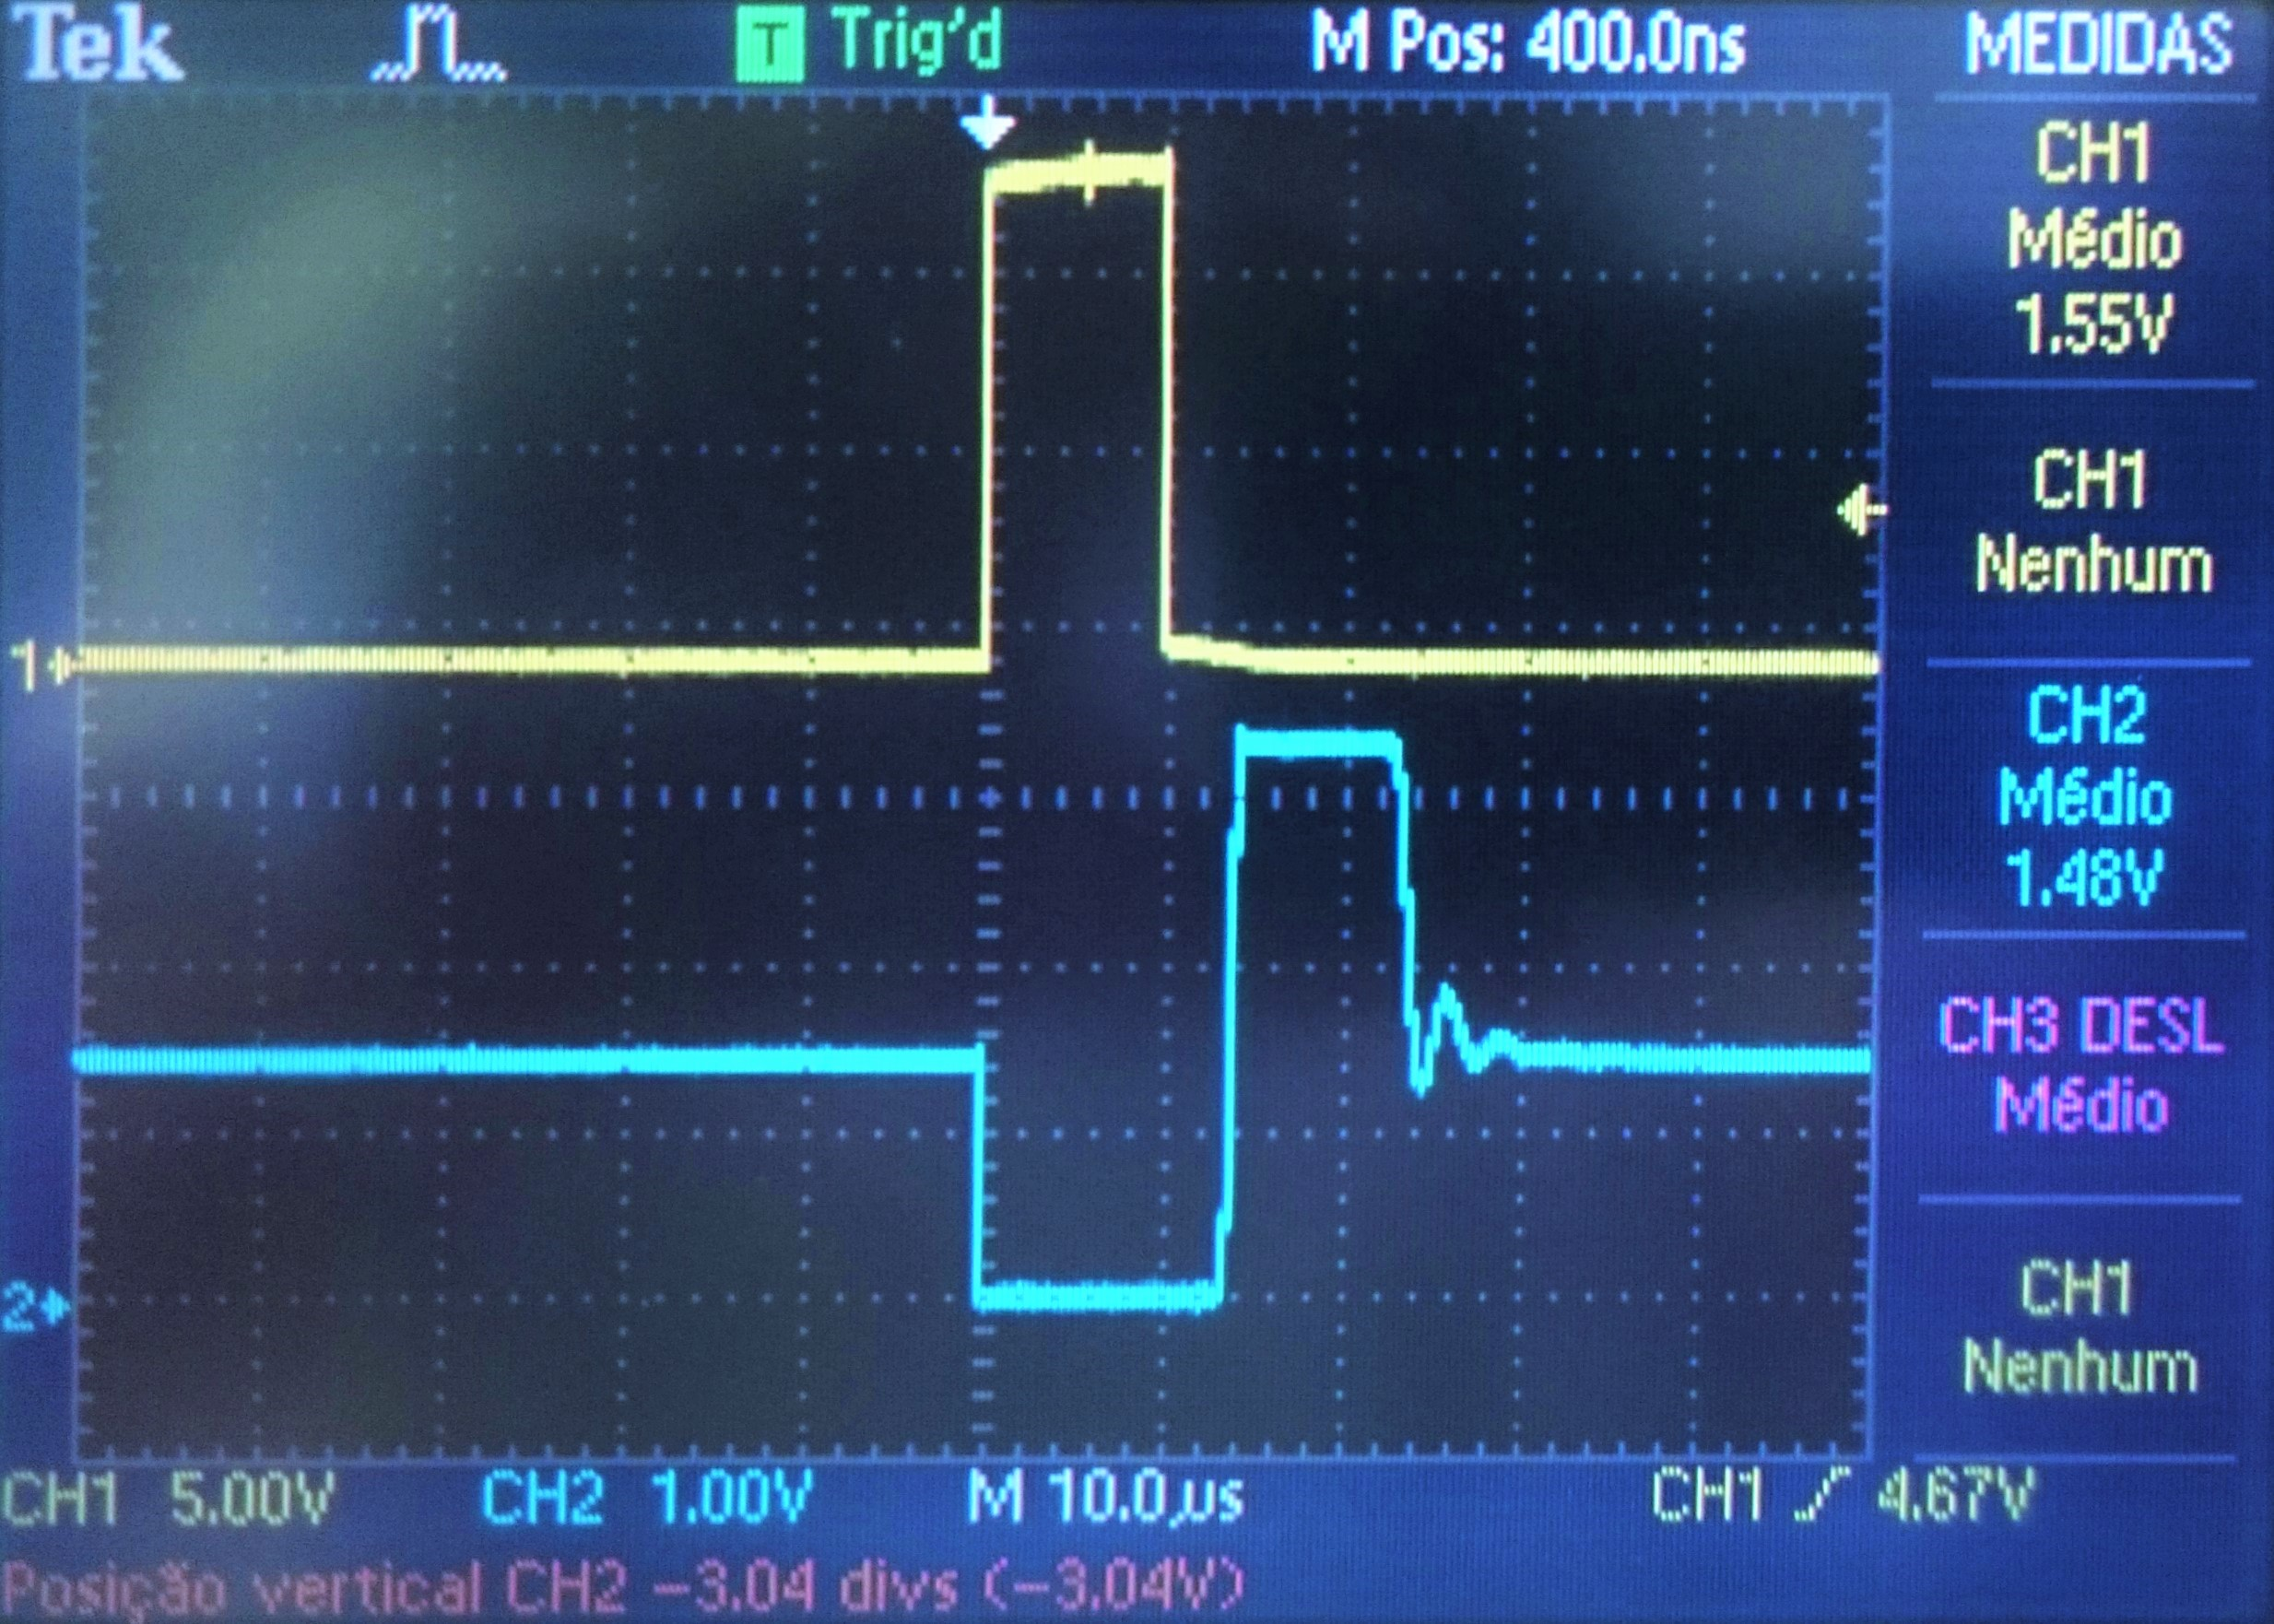
\includegraphics[keepaspectratio=true, scale=0.15]{img/DSC0116}
	\caption{Tensões nos pontos A e B.}
	\label{fig:photo 1}
	\vspace{-0.8em}
\end{figure}

Tem-se assim no canal $1$ (amarelo) a tensão no ponto A e no canal $2$ (azul) a tensão no ponto B. Para o canal 1 observa-se uma onda quadrada de $0$ a aproximadamente $14.8$ V, frequência $2$ kHz e duração de $10$ $\mu$s. O canal $2$, apresenta uma onda retangular com $1,5$ V no qual existe um pico de tensão no flanco ascendente com $3,4$ V estabilizando ao fim de aproximadamente $15$ $\mu$s.

Este pico deve-se a que no momento em que o transístor entra em condução, a bobina encontra-se magnetizada ficando os díodos diretamente polarizado, sendo que a tensão em B será a soma entre a tensão no primário do transformador e Vcc. Após o período de desmagnetização esta estabiliza no valor devido, Vcc. 

Existe também um atraso apreciável entre a tensão em A e B que se deve ao tempo de passagem do transístor da saturação para o corte.

Considera-se agora relevante enunciar a funcionalidade dos díodos presentes no circuito. Em primeiro tem-se o díodo ligado ao primário do transformador cuja função é essencialmente garantir a continuidade da corrente quando o transístor passa ao corte, ficando assim a bobina salvaguardada de potencias descontinuidades na corrente, garantindo o bom funcionamento do circuito. Tem-se ainda o díodo \textit{Zenner} cujo objetivo é diminuir o tempo de desmagnetização da bobina. Isto é devido à superior tensão imposta por este díodo aos terminais do transformador (tensão de \textit{Zenner}), elevando assim a corrente que ali circula. Sendo assim a corrente irá circular nos díodos até que a desmagnetização na bobina seja completada.

A alteração provocada pelo díodo \textit{Zenner} no comportamento do circuito é evidenciada pelas seguintes figuras.

\begin{figure}[h]
	\centering
	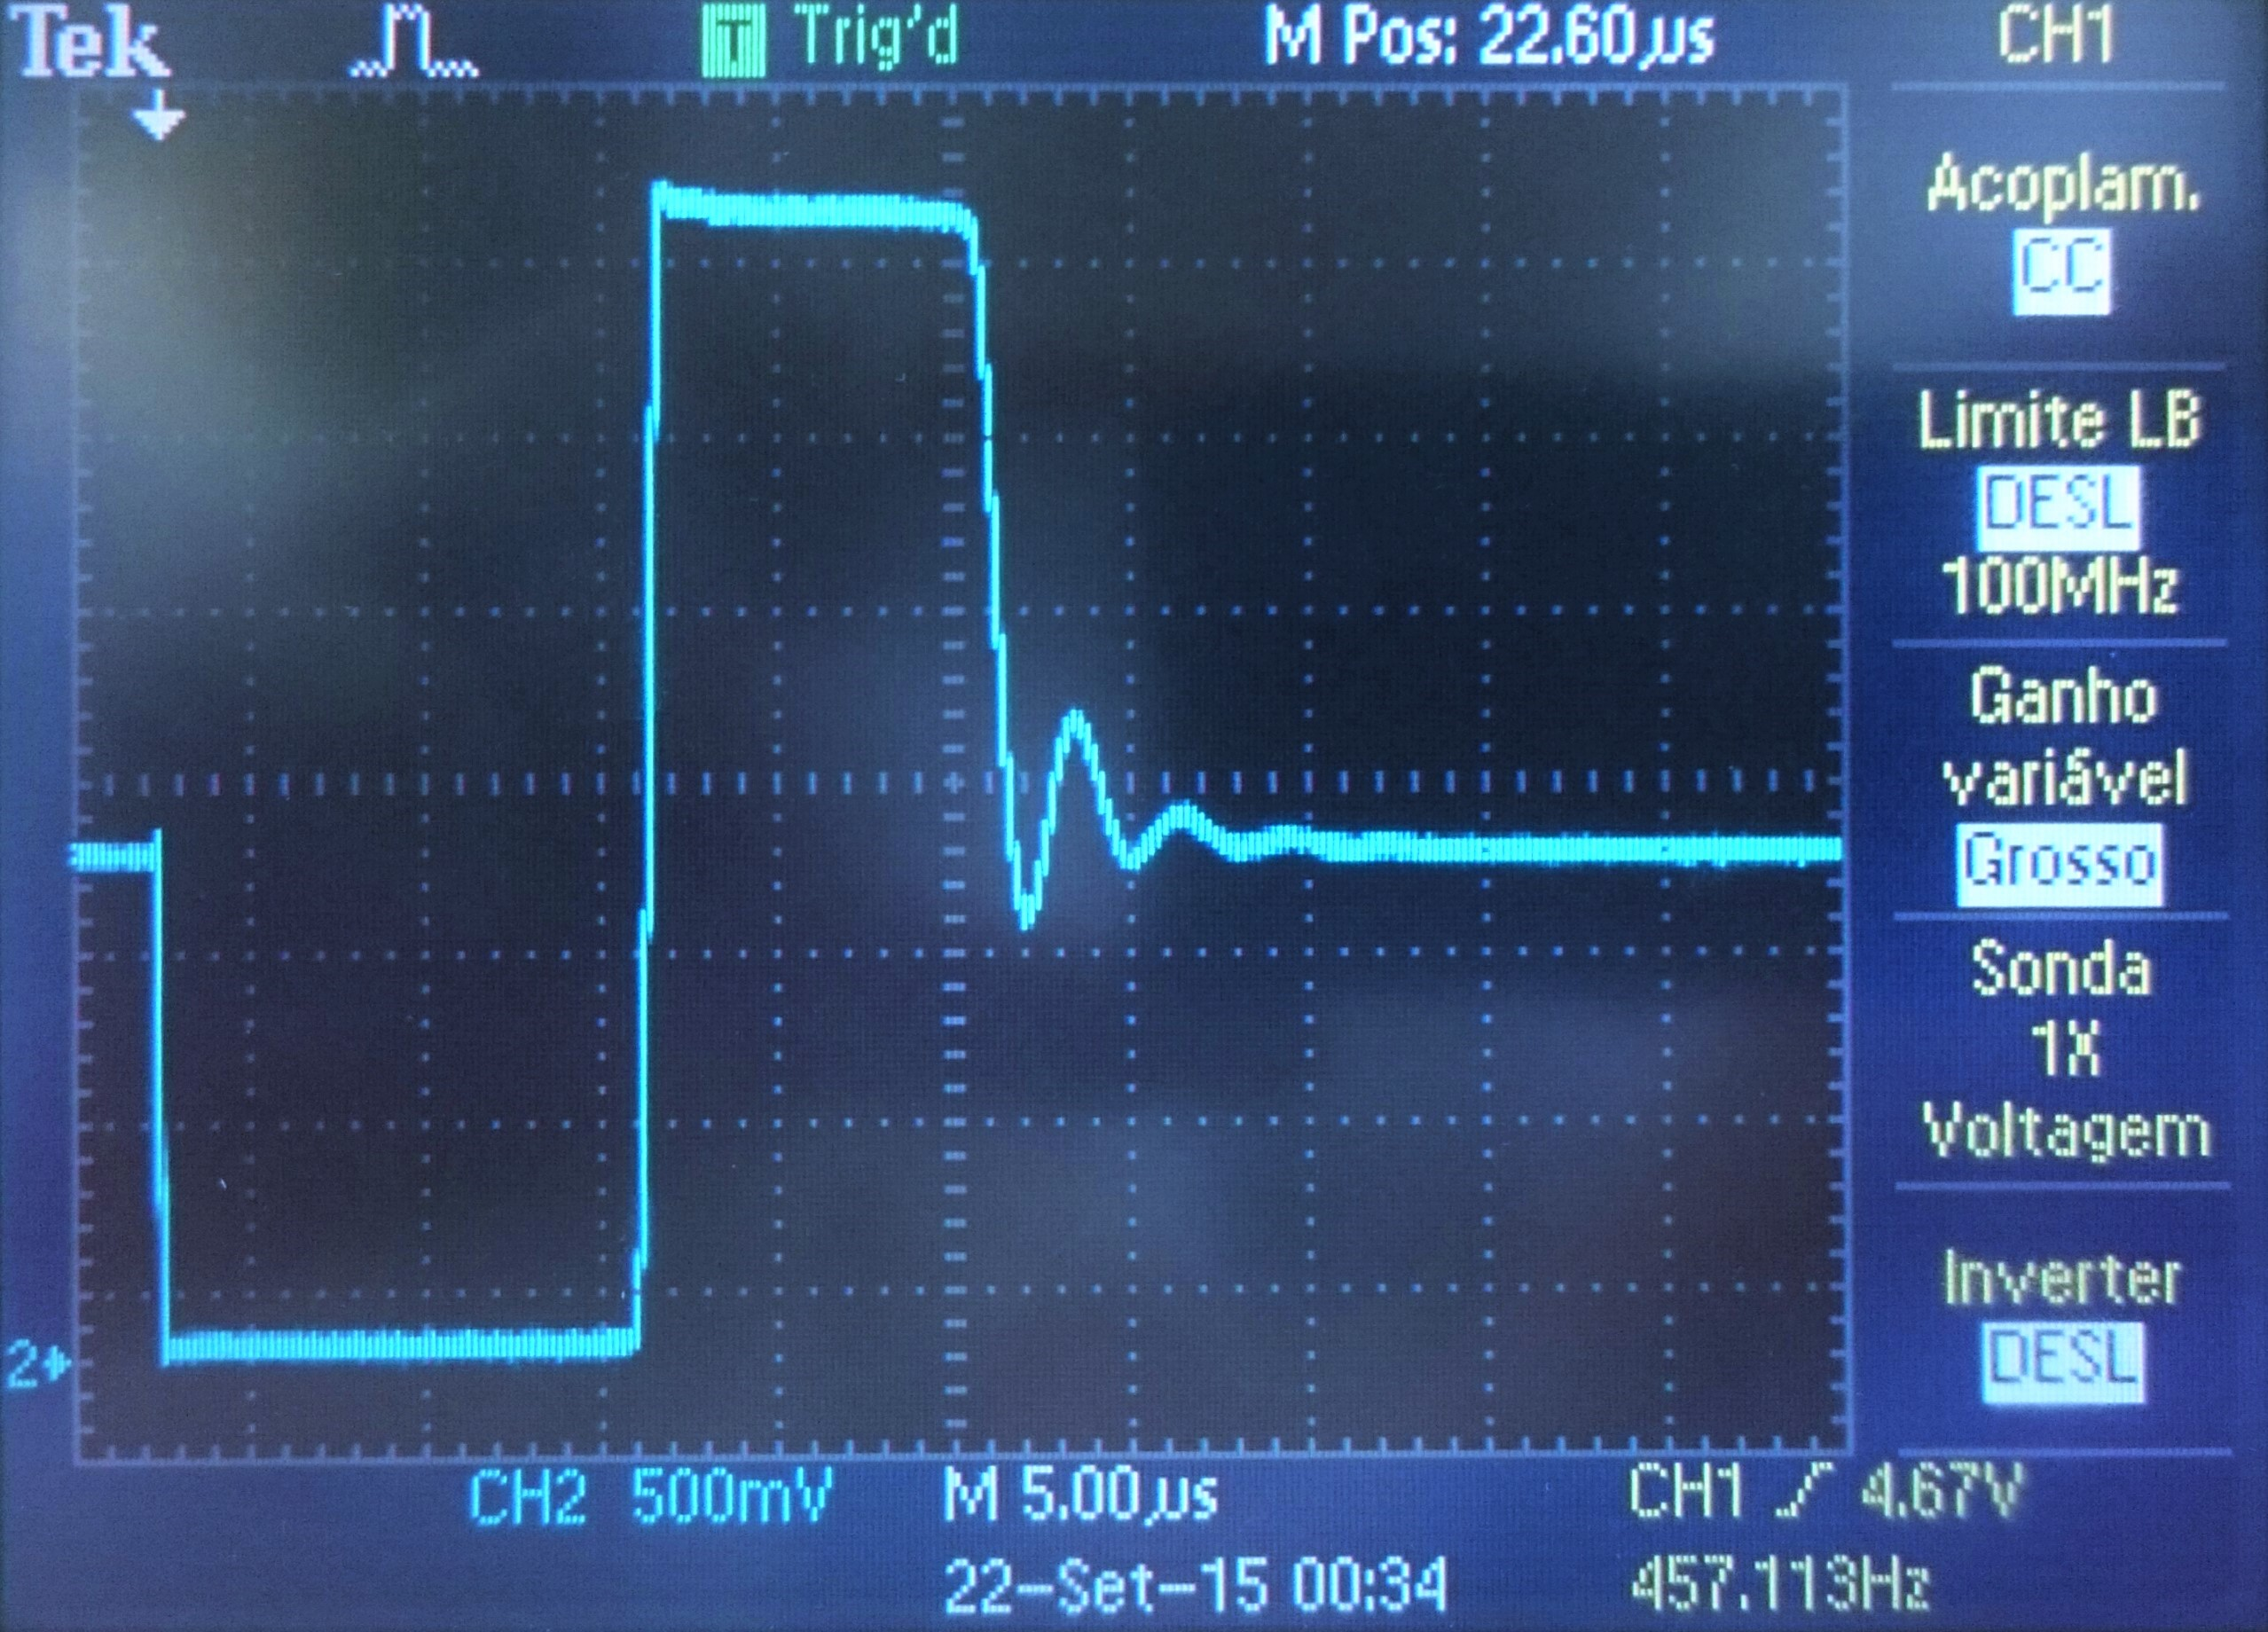
\includegraphics[keepaspectratio=true, scale=0.15]{img/DSC0118}
	\caption{Tensão no ponto B com o díodo \textit{Zenner}.}
	\label{fig:photo 2}
	\vspace{-0.8em}
\end{figure}

\begin{figure}[h]
	\centering
	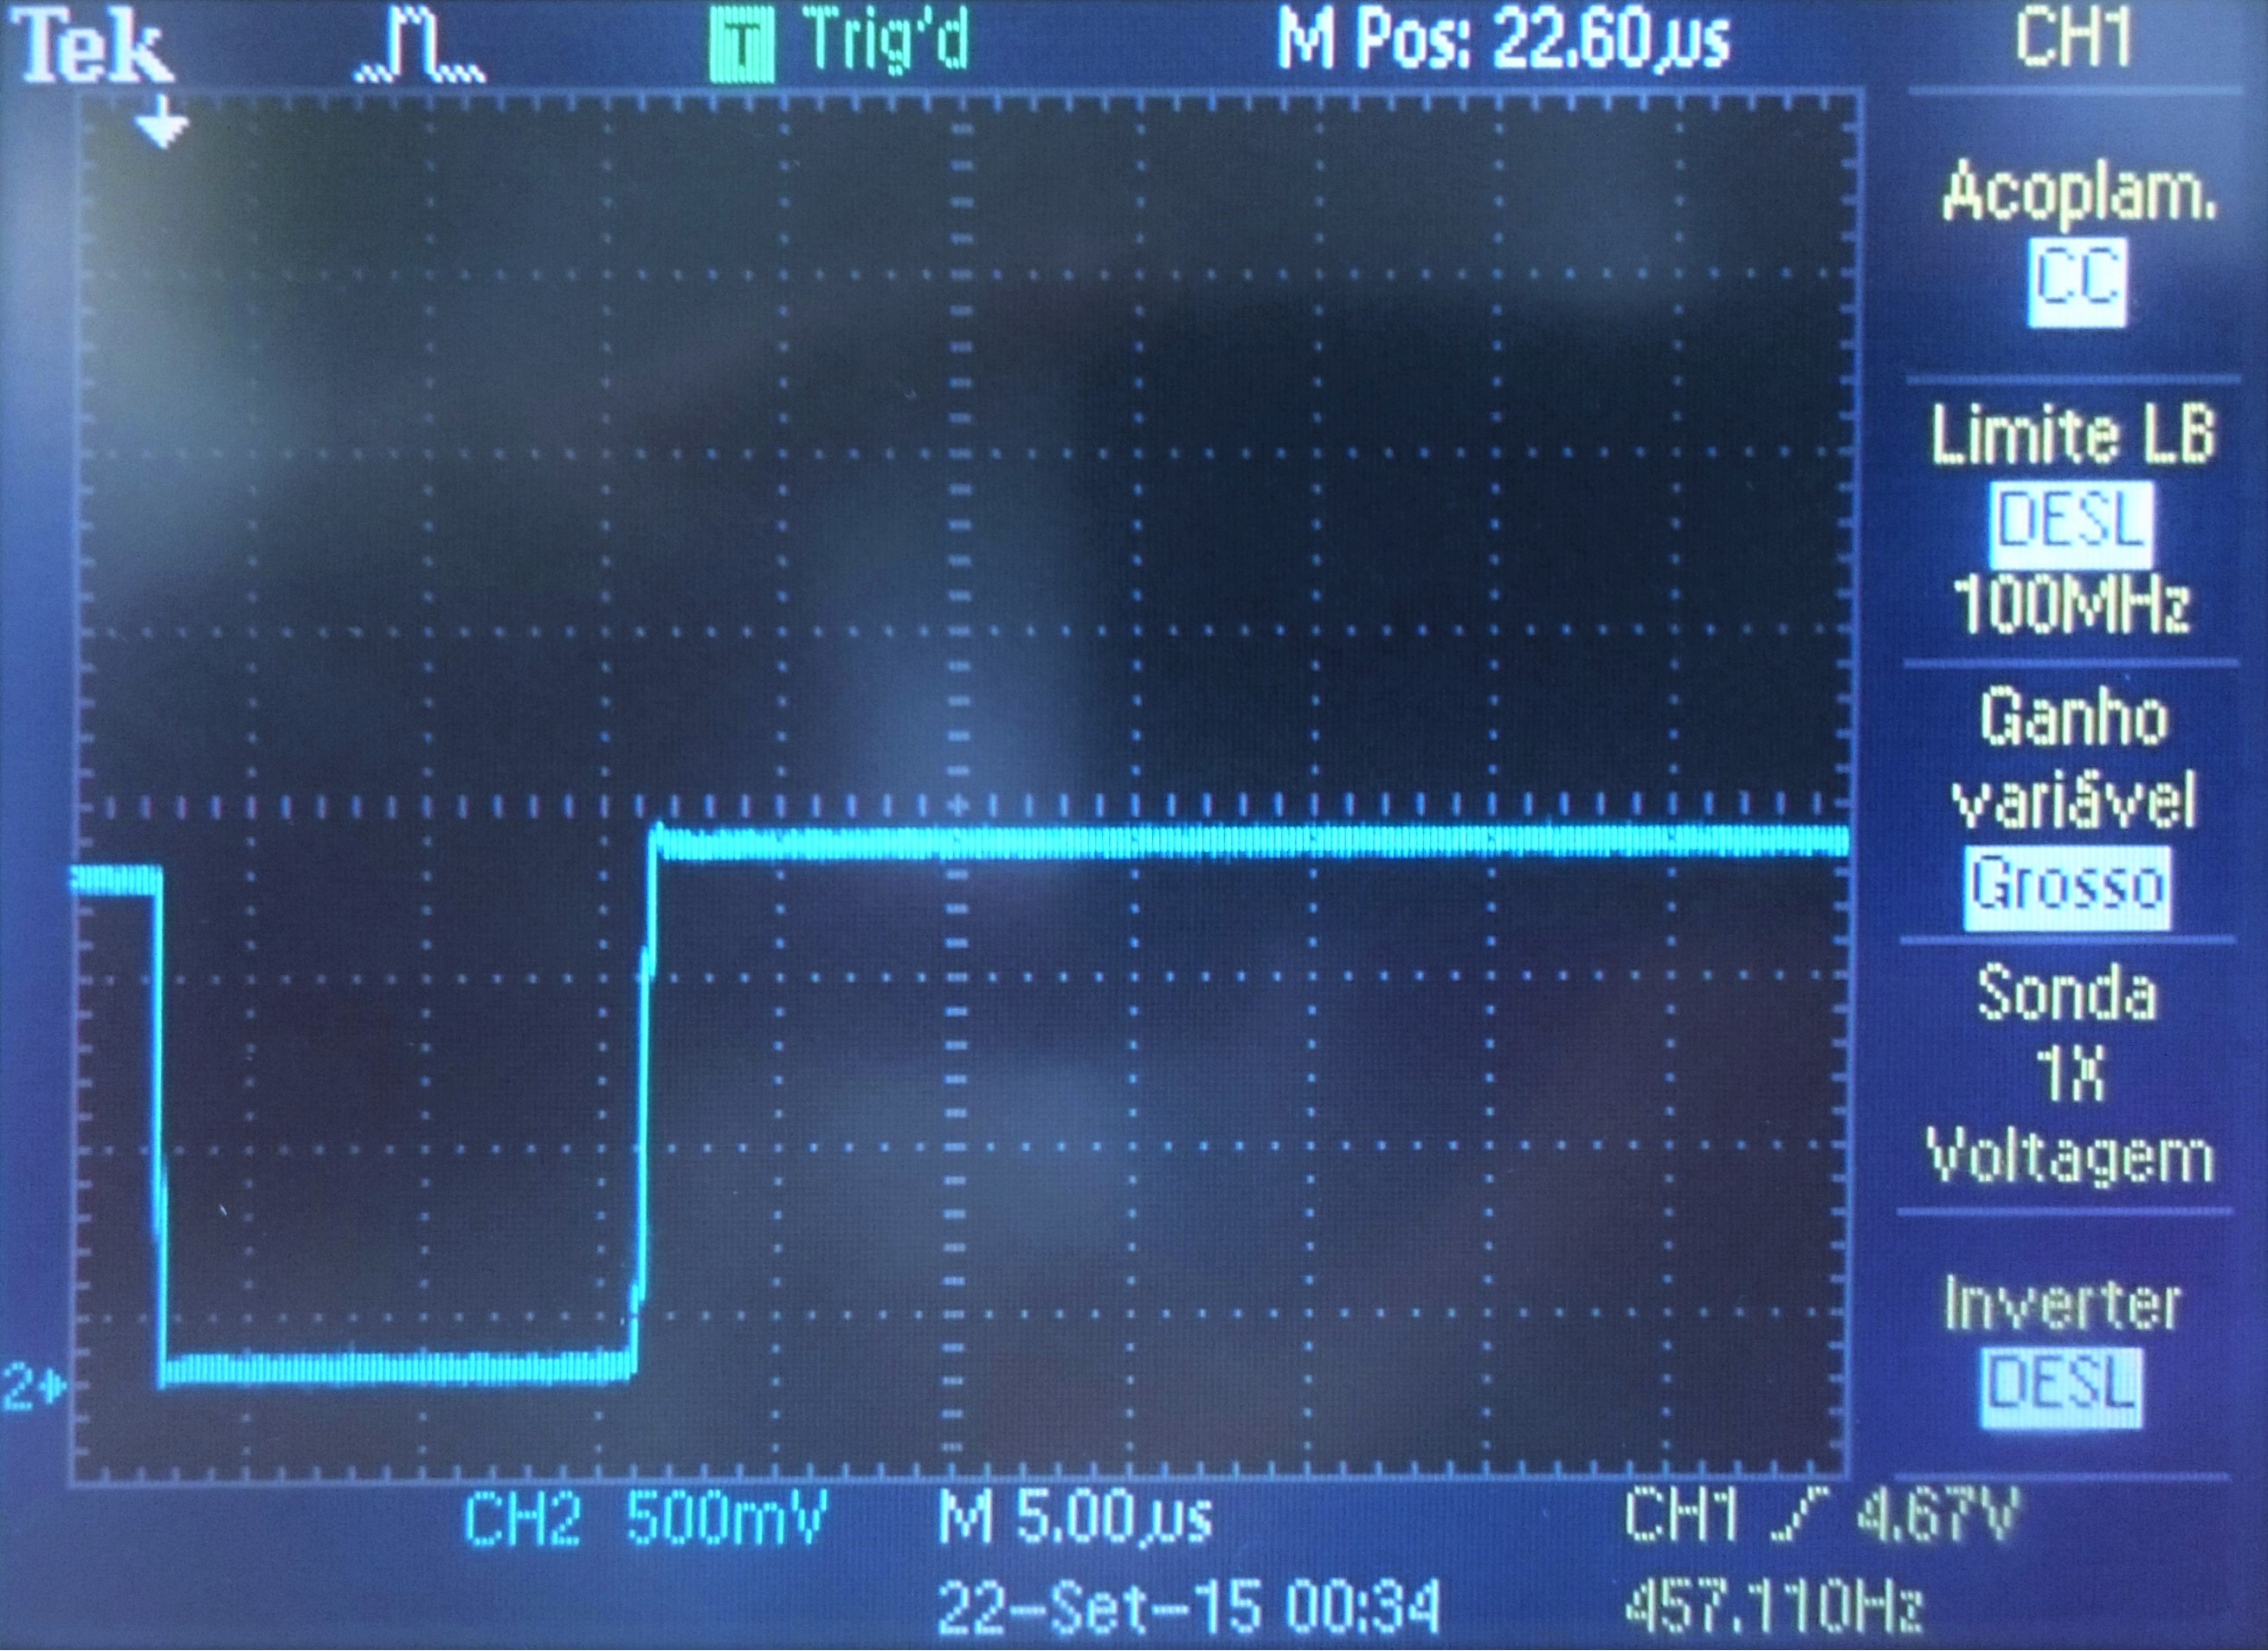
\includegraphics[keepaspectratio=true, scale=0.15]{img/DSC0119}
	\caption{Tensão no ponto B sem o díodo \textit{Zenner}.}
	\label{fig:photo 3}
	\vspace{-0.8em}
\end{figure}

Na \autoref{fig:photo 2} pode concluir-se que o tempo de desmagnetização é relativamente curto, cerca de $30$ $\mu$s em oposição ao tempo de desmagnetização observável na \autoref{fig:photo 3}, onde será mais de $50$ $\mu$s.

A tensão de \textit{Zenner} tem um valor de $-17$ V em oposição à tensão VAK de um díodo normal, $0,7$ V, o que leva a uma dissipação muito mais rápida e por consequência acelera a desmagnetização. Pode observar-se assim graficamente a magnetização pelo área no quadrante positivo e a desmagnetização no quadrante negativo, sendo esta iguais.

 
\end{document}
